\documentclass[10pt]{article}
\usepackage[margin=0.7in]{geometry}
\usepackage{graphicx}
\usepackage{array}
\begin{document}
\begin{center}\Large Projective genus-2 law follow-up\\[3pt]\normalsize Frozen 21-model, 1,260-target paired cohort per arm\end{center}
\noindent\textbf{Scope.} Two complete cold graph-collector arms use the independently checked weighted genus-2 law. The wrapper normalizes every projective output. The state arm keeps weighted divisors across walk steps and normalizes split candidates at the relation boundary. Each arm has 1,260 source-scalar-verified candidate solves and 1,260 same-process, independently source-verified negation-rho solves. The archived wrapped external-law collector is the second comparator. All ratios below divide the summed candidate cost by the summed comparator cost for the same targets.
\medskip
\begin{center}\small\begin{tabular}{r|r r r|r r|r}
Bits & Wrapper/rho & State/rho & State/wrapper & Wrapper/external & State/external & State boundary I \\
\hline
16 & 1.9818 & 1.8665 & 0.9418 & 1.6825 & 1.5846 & 52,444 \\
20 & 2.5346 & 2.5111 & 0.9907 & 1.6571 & 1.6418 & 208,610 \\
24 & 3.3030 & 3.4237 & 1.0365 & 1.6092 & 1.6680 & 672,048 \\
28 & 3.4777 & 3.9598 & 1.1386 & 1.5860 & 1.8059 & 2,811,932 \\
32 & 3.5856 & 3.7514 & 1.0462 & 1.6071 & 1.6815 & 10,275,302 \\
36 & 3.9013 & 4.0603 & 1.0407 & 1.5719 & 1.6359 & 41,087,298 \\
40 & 3.7933 & 4.2482 & 1.1199 & 1.5395 & 1.7241 & 167,267,822 \\
\hline
All & 3.7938 & 4.1793 & 1.1016 & 1.5492 & 1.7067 & 222,375,456 \\
\end{tabular}\end{center}
\noindent Unit: source-addition equivalent (GAE). Representative price: $M+0.5S+10I$ plus 0.1 GAE per native logical operation. Boundary inversion counts are field inversions charged in the state arm; the wrapper's normalization inversions are also charged. Every ratio uses full cold setup, transfer, initialization, relation collection, elimination, and source verification.
\medskip
\noindent Pooled 36-cell wrapper/rho range: 2.0975--21.4887; state/rho range: 1.4729--28.0153. Cells below rho: wrapper 0/36; state 0/36. Pooled state/wrapper range: 0.5468--1.3037; 12/36 prices favor state and 24/36 favor wrapper.
\noindent\textbf{Cold phases.} The standardized cold-phase-breakdown.csv reports arithmetic counts and source-addition-equivalent costs for construction, transfer, walk setup, relation collection and signed elimination, source verification, and a separate row for native logical work. Its phase rows sum to the total representative cost for each arm and comparator, for each bit size and all 1,260 targets.
\begin{center}\small\begin{tabular}{l|r r r r}
40-bit method & Setup & Search/elimination & Native logical & Verification \\
\hline
Wrapper & 1.206 & 2861.016 & 248.087 & 0.079 \\
Weighted state & 0.961 & 3228.833 & 253.458 & 0.079 \\
External & 0.669 & 1771.581 & 248.087 & 0.079 \\
Rho & 0.860 & 734.608 & 84.414 & 0.079 \\
\end{tabular}\end{center}
\noindent Values above are millions of source-addition equivalents for 180 paired 40-bit targets at the representative price. Setup is construction, transfer, and walk initialization, or rho initialization. Full per-size and pooled phase counts are in the CSV.
\begin{center}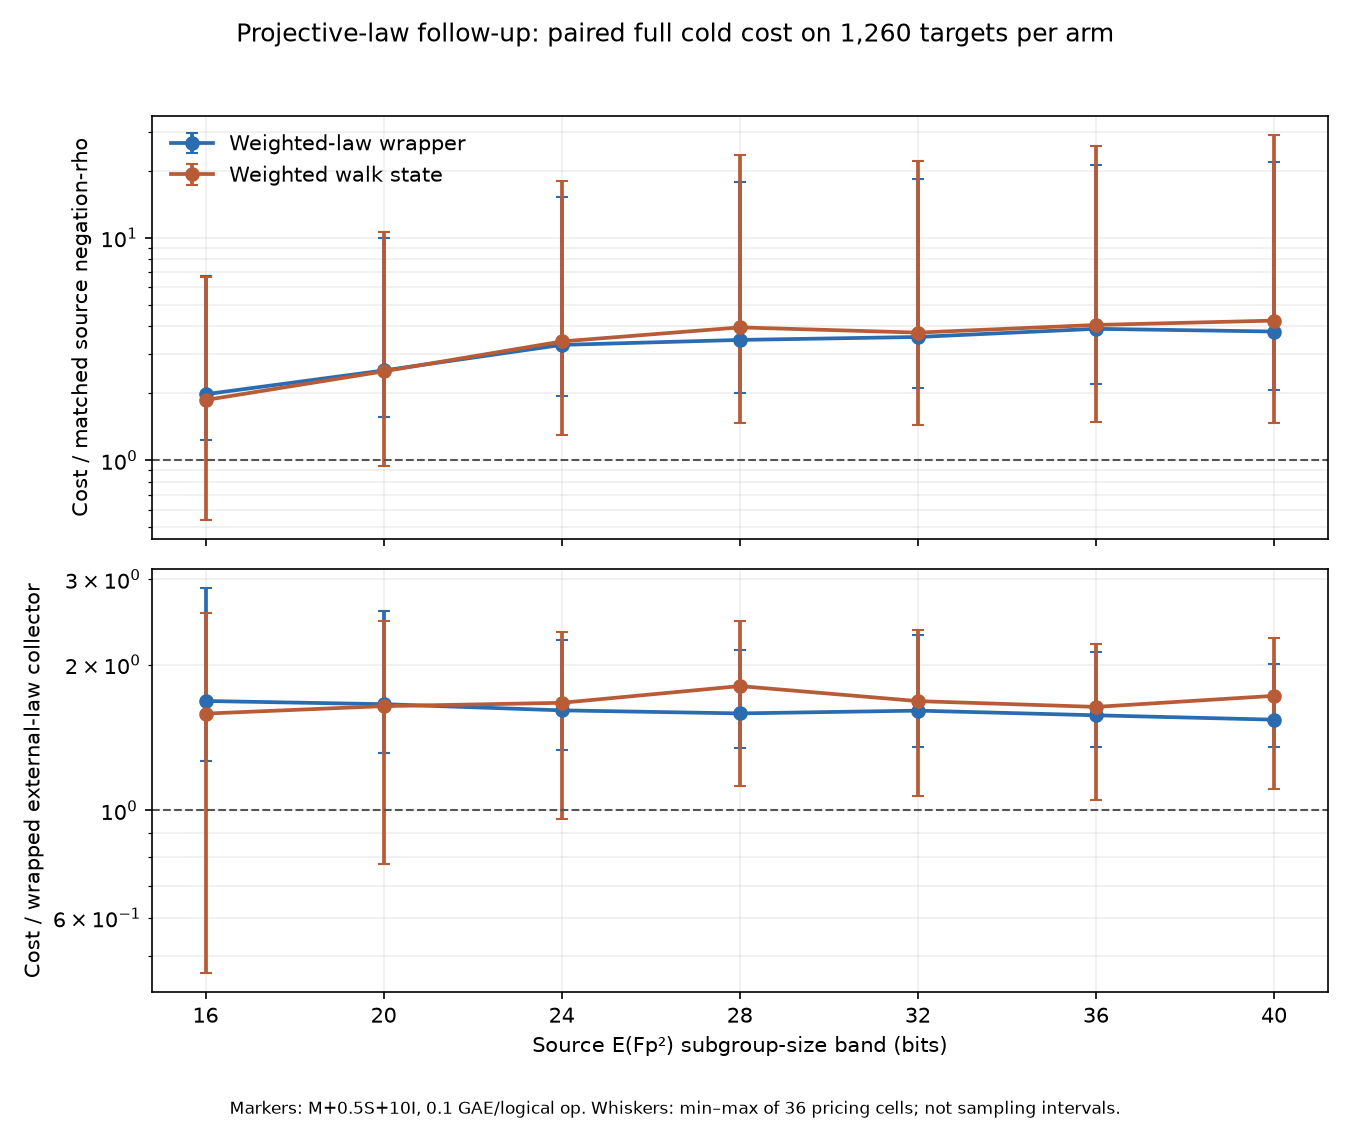
\includegraphics[width=0.95\textwidth]{cost-ratios.png}\end{center}
\begin{center}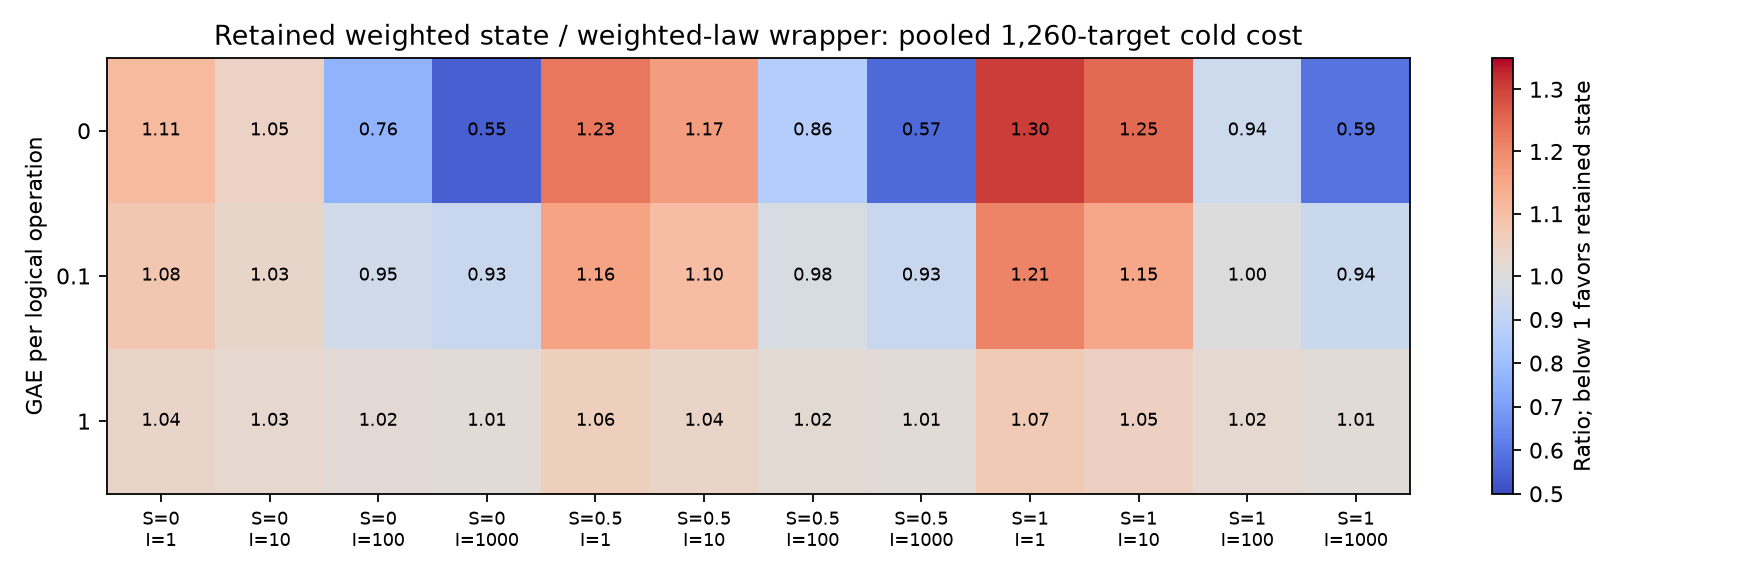
\includegraphics[width=0.95\textwidth]{direct-price-grid.png}\end{center}
\noindent\textbf{Arithmetic gate.} Raw branch records cover all 21 normalized models with non-unit $Z,W$ checks and targeted inverse, coincident-support, degree-drop, and doubling cases. The separate $p=739$ regression preserves the exact input and both $N_6$ variants. These are finite checks, not a proof of universal branch correctness.
\begin{center}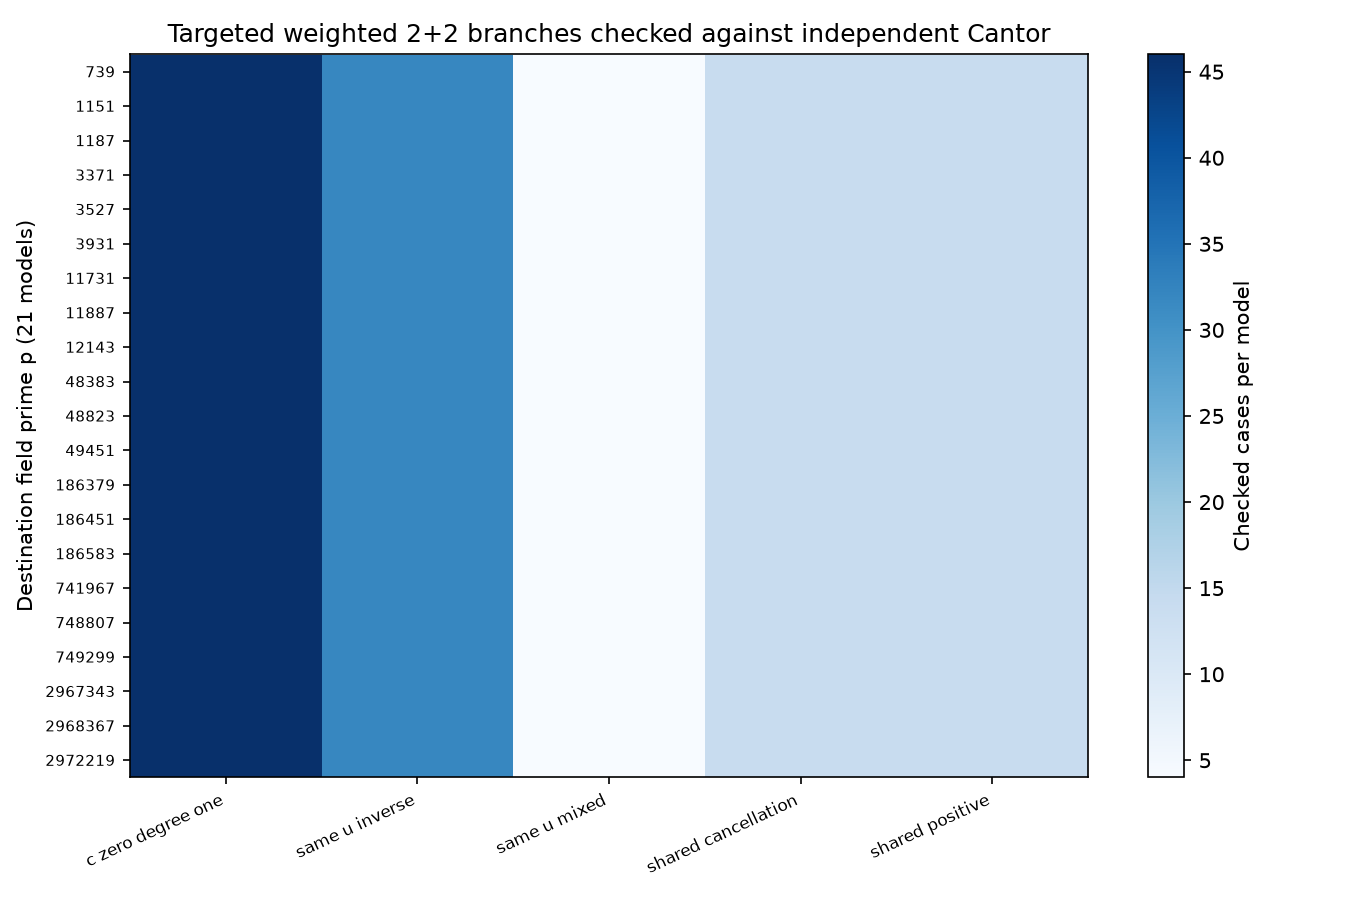
\includegraphics[width=0.85\textwidth]{branch-coverage.png}\end{center}
\medskip
\noindent\textbf{Review files.} PROTOCOL.md defines the cohort and accounting. results/ contains raw per-target JSONL, source-replay and price summaries, both 36-cell grids, and the regression JSON. DATA\_DICTIONARY.md defines every standardized field. VALIDATION\_NOTES.md lists checks and remaining gaps. The SVG and PNG share the same recorded-values source.
\end{document}
